% Options for packages loaded elsewhere
\PassOptionsToPackage{unicode}{hyperref}
\PassOptionsToPackage{hyphens}{url}
%
\documentclass[
]{article}
\usepackage{amsmath,amssymb}
\usepackage{lmodern}
\usepackage{iftex}
\ifPDFTeX
  \usepackage[T1]{fontenc}
  \usepackage[utf8]{inputenc}
  \usepackage{textcomp} % provide euro and other symbols
\else % if luatex or xetex
  \usepackage{unicode-math}
  \defaultfontfeatures{Scale=MatchLowercase}
  \defaultfontfeatures[\rmfamily]{Ligatures=TeX,Scale=1}
\fi
% Use upquote if available, for straight quotes in verbatim environments
\IfFileExists{upquote.sty}{\usepackage{upquote}}{}
\IfFileExists{microtype.sty}{% use microtype if available
  \usepackage[]{microtype}
  \UseMicrotypeSet[protrusion]{basicmath} % disable protrusion for tt fonts
}{}
\usepackage{xcolor}
\usepackage[margin = 0.5in]{geometry}
\usepackage{graphicx}
\makeatletter
\def\maxwidth{\ifdim\Gin@nat@width>\linewidth\linewidth\else\Gin@nat@width\fi}
\def\maxheight{\ifdim\Gin@nat@height>\textheight\textheight\else\Gin@nat@height\fi}
\makeatother
% Scale images if necessary, so that they will not overflow the page
% margins by default, and it is still possible to overwrite the defaults
% using explicit options in \includegraphics[width, height, ...]{}
\setkeys{Gin}{width=\maxwidth,height=\maxheight,keepaspectratio}
% Set default figure placement to htbp
\makeatletter
\def\fps@figure{htbp}
\makeatother
\setlength{\emergencystretch}{3em} % prevent overfull lines
\providecommand{\tightlist}{%
  \setlength{\itemsep}{0pt}\setlength{\parskip}{0pt}}
\setcounter{secnumdepth}{-\maxdimen} % remove section numbering
\newlength{\cslhangindent}
\setlength{\cslhangindent}{1.5em}
\newlength{\csllabelwidth}
\setlength{\csllabelwidth}{3em}
\newlength{\cslentryspacingunit} % times entry-spacing
\setlength{\cslentryspacingunit}{\parskip}
\newenvironment{CSLReferences}[2] % #1 hanging-ident, #2 entry spacing
 {% don't indent paragraphs
  \setlength{\parindent}{0pt}
  % turn on hanging indent if param 1 is 1
  \ifodd #1
  \let\oldpar\par
  \def\par{\hangindent=\cslhangindent\oldpar}
  \fi
  % set entry spacing
  \setlength{\parskip}{#2\cslentryspacingunit}
 }%
 {}
\usepackage{calc}
\newcommand{\CSLBlock}[1]{#1\hfill\break}
\newcommand{\CSLLeftMargin}[1]{\parbox[t]{\csllabelwidth}{#1}}
\newcommand{\CSLRightInline}[1]{\parbox[t]{\linewidth - \csllabelwidth}{#1}\break}
\newcommand{\CSLIndent}[1]{\hspace{\cslhangindent}#1}
\usepackage{caption}
\captionsetup[figure]{font=footnotesize, labelfont=bf}
\usepackage{sectsty}
\usepackage{helvet}
\renewcommand{\familydefault}{\sfdefault}
\usepackage{lineno}
\linenumbers
\renewcommand\linenumberfont{\normalfont\small}
\usepackage{setspace}
\spacing{1.5}
\pagenumbering{arabic}
\usepackage{indentfirst}
\ifLuaTeX
  \usepackage{selnolig}  % disable illegal ligatures
\fi
\IfFileExists{bookmark.sty}{\usepackage{bookmark}}{\usepackage{hyperref}}
\IfFileExists{xurl.sty}{\usepackage{xurl}}{} % add URL line breaks if available
\urlstyle{same} % disable monospaced font for URLs
\hypersetup{
  pdftitle={Erosion of somatic tissue identity with loss of the X-linked intellectual disability factor KDM5C},
  hidelinks,
  pdfcreator={LaTeX via pandoc}}

\title{Erosion of somatic tissue identity with loss of the X-linked
intellectual disability factor KDM5C}
\author{}
\date{\vspace{-2.5em}}

\begin{document}
\maketitle

Gaps in knowledge addressed: * Are other tissue-enriched genes
dysregulated, or only testis, germline genes? * Curating a robust list
of male and female germline genes * Should talk about 2-cell genes vs
germline genes - way to systematically categorize? * Mechanism behind
long-term germline gene misexpression * Recent evidence suggests loss of
KDM5C in ESCs express some germline genes * Unclear if catalytic
activity is required for long-term silencing * Unclear if their
dysregulation lasts throughout life or the same between brain or not *
When in development does it begin? - Recent evidence suggests some
germline genes expressed in 5CKO ESCs but unclear if their dysregulation
lasts throughout differentiation and if the identity of germline genes
are different compared to the brain * Are there functional consequences
to germline gene misexpression?

Introduction: * Chromatin regulators are important for cellular identity
* H3K4me1-3 linked to active gene promoters and enhancers *
Surprisingly, mutations in Chromatin regulators lead to many NDDs
(including many H3K4 regulators) * Recent studies have shown some
chromatin regulators are important for regulating neuron-specific gene
expression/chromatin stat\_compare\_means * However, loss of some
chromatin regulators can also lead to ectopic expression of
tissue-enriched genes * Very few studies have looked at these genes and
it's unclear if these genes contribute to NDD impairments. * Necessary
to first characterize the mechanism behind their derepression to
identify molecular footholds into testing their contribution to neuronal
impairments and potential for therapeutic intervention

\begin{itemize}
\tightlist
\item
  Loss of KDM5C can result in the misexpression of genes typically only
  found in the testis

  \begin{itemize}
  \tightlist
  \item
    Misexpression of tissue-enriched genes hasn't been systematically
    characterized - Unclear if these genes are exceptions or if other
    tissue-specific genes are dysregulated
  \item
    Interestingly, these genes (Cyct, D1pas1) typically function in the
    germline
  \item
    Germ cells (meiotic cells) are typically distinguished from somatic
    cells very early on in embyrogenesis and is a key feature of
    multicellularity
  \item
    Chromatin regulators are very important for decommissioning germline
    genes and act successively the embryo implants into the uterine wall

    \begin{itemize}
    \tightlist
    \item
      Most studies have focused on ESCs, which have a similar
      transcriptome to germ cells / 2-cells
    \item
      recently, KDM5C was shown to repress DAZL in ESCs, independent of
      its catalytic activity
    \item
      However, DNA methylation is lost in the mature 5CKO brain, DNA
      methylation is placed later and it's Unclear if it's required for
      long-term repression (maybe too specific, just trying to go into
      the fact that the mechanism is partially understood but unclear)
    \end{itemize}
  \item
    Systematic characterization of ectopic germline genes hasn't been
    done

    \begin{itemize}
    \tightlist
    \item
      unknown if other germline-enriched genes are dysregulated,
      including oocyte-specific genes
    \item
      Crucially, it's unknown if misexpression of the germline program
      leads to functional consequences in 5CKO cells.
    \end{itemize}
  \end{itemize}
\end{itemize}

\hypertarget{introduction}{%
\section{Introduction}\label{introduction}}

To form a complete organism, embryonic stem cells must differentiate
into a myriad of discrete cellular identities. This is in part
accomplished by chromatin regulators that can either promote or impede
lineage-specific gene expression through histone and DNA
modifications\textsuperscript{1,2}. Although initially identified for
their roles in cellular identity\textsuperscript{3,4}, recent
advancements in next generation sequencing technologies unexpectedly
found many neurodevelopmental disorders (NDDs) are caused by or linked
to mutations in chromatin regulators. This relationship is partially
explained by their regulation of brain-specific genes or chromatin
states, such as modulating genes involved in synaptic
maturation\textsuperscript{5} or the transition between neuronal and
glial developmental programs\textsuperscript{6}. However, loss of some
chromatin regulators can also lead to the misexpression of
tissue-specific genes outside of their intended
environment\textsuperscript{3,4,7}. Currently, very few studies have
explored the misexpression of non-neuronal, tissue-specific genes in
chromatin-linked neurodevelopmental disorders\textsuperscript{8,9} and
it is unclear if this partial loss of brain identity contributes to
neurodevelopmental impairments. To elucidate their contribution to
neurodevelopmental impairments, it is essential to first characterize
the types of genes misexpressed, the developmental time point the
dysregulation begins, and the molecular mechanism underlying their
de-repression. Characterizing these features will enable us to identify
molecular footholds common between NDDs that can then be exploited for
potential therapeutics.

In this study, we characterized the misexpression of tissue-enriched
genes with loss of the chromatin regulator lysine demethylase 5C (KDM5C,
also known as SMCX or JARID1C), a histone 3 lysine 4 demethylase.
Pathogenic mutations in \emph{KDM5C} cause Intellectual Developmental
Disorder, X-linked, Syndromic, Claes-Jensen Type (MRXSCJ, OMIM: 300534),
whose features include short stature, intellectual disability, seizures,
aberrant aggression, and autistic behaviors\textsuperscript{10--12}.
Previous work has demonstrated constitutive \emph{Kdm5c} knockout (-KO)
mice recapitulate key MRXSCJ patient phenotypes, including
hyperaggression and learning impairments\textsuperscript{13}. Next
generation RNA sequencing (RNA-seq) in the \emph{Kdm5c}-KO hippocampus
unexpectedly revealed ectopic expression of testis-enriched genes within
the brain\textsuperscript{9}. However, it is currently unclear if
misexpression in the \emph{Kdm5c}-KO brain is unique to testis genes, as
other tissue-enriched genes have not been systematically evaluated.

Interestingly, some of the ectopic testis transcripts identified in the
\emph{Kdm5c}-KO brain are typically expressed in germ
cells\textsuperscript{9}. Unlike somatic cells, germ cells (e.g.~sperm
and eggs) undergo meiosis and pass on their genetic material to the next
generation. The germline and the soma are typically distinguished during
early embryogenesis, when germline genes are silenced in epiblast stem
cells soon after implantation and only reactivated in a subset to form
the germline. Chromatin regulators play a key role in decommissioning
germline genes as the embryo transitions from naive to primed
pluripotency by placing repressive histone H2A lysine 119
monoubiquitination (H2AK119ub1)\textsuperscript{14}, histone 3 lysine 9
trimethylation (H3K9me3)\textsuperscript{14,15}, and DNA CpG
methylation\textsuperscript{15--17} at germline gene promoters. KDM5C
may also be involved in this early decommissioning of germline genes, as
re-expression of KDM5C in neurons fails to surpress their
dysregulation\textsuperscript{9}. In support of this, KDM5C was very
recently shown to repress \emph{Deleted in azoospermia like (Dazl)}, a
key regulator of germline development, in mouse embryonic stem cells
(ESCs)\textsuperscript{18,19}. In support of this, two independent
screens in mouse embryonic stem cells (ESCs) recently identified KDM5C
as a repressor of \emph{Deleted in azoospermia like (Dazl)}, a key
regulator of germline development. However, KDM5C's role in embryonic
germline gene repression is currently unclear, given that Dazl is also
expressed in ESCs and in the 2-cell stage and germline gene
misexpression has yet to be globally characterized during
\emph{Kdm5c}-KO embryogenesis.

To elucidate KDM5C's role in tissue identity, here we characterized the
aberrant transcription of tissue-enriched genes within the
\emph{Kdm5c}-KO brain and epiblast-like cells (EpiLCs), an \emph{in
vitro} model of the post-implantation embryo. We identified general
dysregulation of tissue-enriched genes in both the adult \emph{Kdm5c}-KO
brain and EpiLCs, including misexpression of liver, muscle, and ovary
genes. The \emph{Kdm5c}-KO amygdala and hippocampus had significant
enrichment of testis-biased genes that are unique to germ cells. To
better characterize germline gene misexpression, we then generated a
dataset of germline-enriched genes by comparing gene expression in
gonads with germ cell depletion. We found \emph{Kdm5c}-KO EpiLCs
primarily expressed unique germline genes compared to the mature
\emph{Kdm5c}-KO brain, including \emph{Dazl} and \emph{Stra8}, key
drivers of germline identity and meiosis. While KDM5C is directly bound
to some germline gene promoters in EpiLCs, it is not directly bound to
many germline-enriched mRNAs expressed with \emph{Kdm5c}-KO cells,
indicating germline genes can be aberrantly transcribed through indirect
mechanisms. Finally, we found KDM5C loss impairs the placement of DNA
methylation at germline gene promoters as ESCs differentiate into
EpiLCs. Therefore, we propose KDM5C plays a crucial role in the
development of tissue identity during early embryogenesis, including
establishment of the soma-germline boundary.

\textbf{note: need a better conclusion sentence - work on when we know
what's happening with last figure/functional consequences}

\hypertarget{results}{%
\section{Results}\label{results}}

\hypertarget{tissue-enriched-genes-including-testis-genes-are-aberrantly-expressed-in-the-kdm5c-ko-brain}{%
\subsection{\texorpdfstring{Tissue-enriched genes, including testis
genes, are aberrantly expressed in the \emph{Kdm5c}-KO
brain}{Tissue-enriched genes, including testis genes, are aberrantly expressed in the Kdm5c-KO brain}}\label{tissue-enriched-genes-including-testis-genes-are-aberrantly-expressed-in-the-kdm5c-ko-brain}}

\begin{itemize}
\tightlist
\item
  \textbf{note: should I compare amygdala and hippocampus? scandaglia
  only looked at hippocampus}
\end{itemize}

Previous RNA sequencing (RNA-seq) in the adult hippocampus ectopic
expression of some testis genes within the \emph{Kdm5c} knockout (-KO)
brain\textsuperscript{9}. Since tissue-enriched genes have not been
systematically characterized in the \emph{Kdm5c}-KO brain, it is
currently unclear if this erosion of brain tissue identity is a major
consequence of \emph{Kdm5c} loss and if it is unique to testis-enriched
genes. Therefore, we first globally assessed the expression of
previously characterized mouse tissue-enriched genes\textsuperscript{20}
in our published mRNA-seq datasets of the amygdala and hippocampus in
adult mice with constitutive knockout of
\emph{Kdm5c}\textsuperscript{21}.

We found a large proportion of genes significantly upregulated within
the \emph{Kdm5c}-KO brain (DESeq2\textsuperscript{22}, log2 fold change
\textgreater{} 0.5, q \textless{} 0.1) are typically enriched in
non-brain tissues (Amygdala: 35\%, Hippocampus: 24\%) (Figure 1A-B). The
majority of tissue-enriched differentially expressed genes
(tissue-enriched DEGs) were testis genes (Figure 1A-C). Testis-biased
DEGs were significantly enriched for both brain regions (Amygdala p =
1.83e-05; Hippocampus p = 4.26e-11, Fisher's Exact Test), even though
the testis has the largest total number of tissue-biased genes compared
to any other tissue (2,496 genes). Of note, we did not observe
enrichment of brain-enriched genes (Amygdala p = 1; Hippocampus p =
0.74, Fisher's Exact), despite the fact these are brain samples and the
brain has the second highest total number of tissue-enriched genes (708
genes).

In addition to the high enrichment of testis genes, we also identified
aberrant expression of other tissue-enriched genes within the
\emph{Kdm5c}-KO brain. Although the \emph{Kdm5c}-KO mice were male, we
also observed significant enrichment of ovary-biased DEGs in both the
amygdala and hippocampus (Amygdala p = 0.00574; Hippocampus p = 0.048,
Fisher's Exact) (Figure 1D). Intriguingly, many ovary and testis-biased
DEGs have functions specific to germ cells and have no known role in the
brain. For example, the testis-biased DEG \emph{FK506 binding protein 6
(Fkbp6)} is a known regulator of piRNA expression and meiosis in germ
cells\textsuperscript{23,24} (Figure 1C) while the ovary-enriched DEG
\emph{Zygotic arrest 1 (Zar1)} was recently shown to sequester mRNAs in
oocytes for meiotic maturation and early zygote
development\textsuperscript{25} (Figure 1D). Although not consistent
across brain regions, we also found enrichment of two non-gonadal
tissues - the liver (Amygdala p = 0.0398, Fisher's Exact Test) and the
muscle (Hippocampus p = 0.0104, Fisher's Exact Test). An example of a
liver-biased DEG is \emph{Apolipoprotein C-I (Apoc1)}, which is involved
in lipoprotein metabolism (Figure 1E). Testis, ovary, and liver-enriched
DEGs showed little to no expression in the wild-type brain, yet our
mRNA-seq data indicate they are polyadenylated and spliced into mature
transcripts (Figure 1C-E). Together, these results suggest misexpression
of testis and other tissue-enriched genes within the brain is a major
effect of KDM5C loss.

\hypertarget{germline-genes-are-aberrantly-expressed-in-the-male-kdm5c-ko-brain}{%
\subsubsection{\texorpdfstring{Germline genes are aberrantly expressed
in the male \emph{Kdm5c}-KO
brain}{Germline genes are aberrantly expressed in the male Kdm5c-KO brain}}\label{germline-genes-are-aberrantly-expressed-in-the-male-kdm5c-ko-brain}}

The testis contains both germ cells (meiotic cells, e.g.~spermatogonia)
and somatic cells (non-meiotic, e.g.~Leydig cells) that support hormone
production and germline functions. Select testis-enriched DEGs that were
characterized previously had germline-specific
functions\textsuperscript{9}, suggesting \emph{Kdm5c}-KO cells fail to
demarcate between the soma and germline. To test if this holds true for
all \emph{Kdm5c}-KO testis-biased DEGs, we first assed their function
through gene onotology. We found high enrichment of germline-relevant
ontologies, including spermatid development (GO: 0007286, p.adjust =
6.2e-12) and sperm axoneme assembly (GO: 0007288, p.adjust = 2.45e-14)
(Figure 2A).

To further validate if these testis DEGs are truly germline genes, we
then compared their expression in somatic versus germ cells within the
testis. We first compared their expression within wild-type versus germ
cell-depleted testes\textsuperscript{26}. In this study, germ cell
depletion was accomplished by heterozygous \emph{W} and \emph{Wv}
mutations in the enzymatic domain of \emph{c-Kit}
(Kit\textsuperscript{W/Wv}), which prevents the maturation of germ cells
and results in overall germline loss\textsuperscript{27}. Almost all
\emph{Kdm5c}-KO testis-enriched DEGs lost expression with germ cell
depletion (Figure 2B). The only testis-enriched DEG that did not show
considerable downregulation with germline depletion was \emph{FK506
binding protein 6 (Fkbp6)}, the aforementioned testis gene that
regulates piRNA expression and meiosis in germ
cells\textsuperscript{23,24}. We then assessed testis-enriched DEG
expression in a published single cell RNA-seq dataset that identified
cell type-specific markers within the testis\textsuperscript{28}. We
found that while some testis-enriched DEGs were classified as specific
markers for different germ cell types (e.g.~spermatogonia,
spermatocytes, round spermatids, and elongating spermatids) none marked
somatic cells (Figure 2C). Together, these data suggest the somatic
\emph{Kdm5c}-KO brain aberrantly expresses germline genes.

We wanted to more deeply characterize germline gene misexpression with
\emph{Kdm5c} loss, but lacked a comprehensive list of mouse
germline-enriched genes. To facilitate downstream analyses, we generated
a list of male and female germline-enriched genes by evaluating gene
expression in germline-depleted (Kit\textsuperscript{W/Wv}) mice.
Current available Kit\textsuperscript{W/Wv} datasets included males and
females at embryonic day 12, 14, and 16\textsuperscript{29}, as well as
adult male testes\textsuperscript{26}.

We defined genes as germline-enriched if their expression met the
following criteria: 1) their expression is greater than 1 FPKM in
wild-type gonads 2) their expression in any wild-type, non-gonadal
tissue\textsuperscript{20} does not exceed 20\% of their maximum
expression in the wild-type germline, and 3) their expression in the
germ cell-depleted germline, for any sex or time point, does not exceed
20\% of their maximum expression in the wild-type germline. These
criteria yielded 1,288 germline-enriched genes (Figure 2D), which was
hereafter used as a resource for assessing misexpression of germline
genes with loss of \emph{Kdm5c} (Supplementary table 1).

\hypertarget{kdm5c-ko-epiblast-like-cells-aberrantly-express-master-regulators-of-germline-identity}{%
\subsection{\texorpdfstring{\emph{Kdm5c}-KO epiblast-like cells
aberrantly express master regulators of germline
identity}{Kdm5c-KO epiblast-like cells aberrantly express master regulators of germline identity}}\label{kdm5c-ko-epiblast-like-cells-aberrantly-express-master-regulators-of-germline-identity}}

Misexpression of germline genes in the adult \emph{Kdm5c}-KO brain
suggests mutants fail to demarcate germline and somatic cellular
identity. Germ cells are typically distinguished from somatic cells soon
after the embryo implants into the uterine wall\textsuperscript{30,31}
when a subset of epiblast stem cells become the primordial germ cells
(PGCs) while the remainder differentiate into the ectoderm, mesoderm,
and endoderm to form the somatic tissues\textsuperscript{32}. This
developmental time point can be modeled \emph{in vitro} through
differentiation of embryonic stem cells (ESCs) into post-implantation
epiblast-like stem cells (EpiLCs) (Figure 3A, top). Previous studies
have demonstrated that while some germline-enriched genes are also
expressed in embryonic stem cells (ESCs), they are silenced as they
differentiate into EpiLCs\textsuperscript{15}. Therefore, we assessed if
KDM5C was necessary for initial germline gene silencing by evaluating
the impact of \emph{Kdm5c} loss in male EpiLCs.

We first identified \emph{Kdm5c}-KO EpiLC DEGs through DESeq2 analysis
of our previously published RNA-seq dataset\textsuperscript{33} (log2
fold change \textgreater{} 0.5, q \textless{} 0.1). Similar to the
\emph{Kdm5c}-KO brain, we observed general dysregulation of
tissue-enriched genes, with the largest number of genes belonging to the
brain and testis, although they were not significantly enriched (Figure
3B). Using our curated list, we found \emph{Kdm5c}-KO EpiLCs aberrantly
expressed 54germline-enriched genes, including the previously
characterized hippocampal DEG\textsuperscript{9} \emph{Cytochrome C,
testis-specific (Cyct)} (Figure 3C). Although we observed aberrant
expression of many tissue-enriched genes, we did not observe any
significant difference in primed pluripotency genes (Figure 3D) or gross
changes in \emph{Kdm5c}-KO cell morpholgy during differentiation (Figure
3E), indicating KDM5C loss does not impair EpiLC formation.

To evaluate if all germline DEGs are constitutively dysregulated or
change over the course of development, we then compared EpiLC germline
DEGs to those expressed in the \emph{Kdm5c}-KO brain. The majority of
EpiLC germline DEGs were unique to EpiLCs, with only \emph{Cyct} shared
across all sequencing datasets (Figure 3F). We then compared the
function of EpiLC and brain germline DEGs and found particularly high
enrichment of meiosis-related gene ontologies in EpiLCs (Figure 3G),
such as meiotic cell cycle (GO: 0051321, p.adjust = 4.44e-07). While
there was modest enrichment of meiotic gene ontologies in in both brain
regions, the \emph{Kdm5c}-KO hippocampus showed strong enrichment of
late-stage sperm genes, such those involved in the sperm axoneme. This
shift from meiotic genes to later spermatogenesis genes in the
hippocampus suggests the germline developmental program could occur
ectopically as \emph{Kdm5c}-KO cells progresses through somatic tissue
development. \textbf{note: this is strengthened by the ChIP-seq data
since KDM5C is not directly bound to many brain/flagellar DEGs.This
point might be stronger in the ChIPseq figure}

Interestingly, DEGs unique to \emph{Kdm5c}-KO EpiLCs included key
drivers of germline identity, such as \emph{Stimulated by retinoic acid
8 (Stra8)} and \emph{Deleted in azoospermia like (Dazl)} (Figure 3H).
These genes are typically expressed during embryonic germ cell
development to commit PGCs to the germline fate, but are also expressed
later in life to trigger meiotic gene expression
programs\textsuperscript{34--36}. Of note, some germline genes,
including \emph{Dazl}, are also expressed in the two-cell embryo.
However, we did not see misexpression of two-cell embryo-specific genes,
like \emph{Zscan4d} (q = 0.381), indicating \emph{Kdm5c}-KO in EpiLCs do
not revert back to a 2-cell state (Figure 3H).

\emph{Dazl} is an RNA-binding protein that regulates the translation of
germline mRNAs and is essential for germ cell
function\textsuperscript{37}. A significant portion of germline
transcripts misexpressed in \emph{Kdm5c}-KO EpiLCs are known binding
targets of DAZL, including \emph{Stra8}\textsuperscript{38} (p =
1.698e-07, Fisher's Exact Test). This suggests expression of DAZL
protein could promote the translation of other aberrant germline
transcripts, influencing their ability to impact \emph{Kdm5c}-KO
cellular function. We thus tested DAZL protein expression in
\emph{Kdm5c}-KO EpiLCs through immunocytochemistry (Figure 3H). We
observed about 25\% of \emph{Kdm5c}-KO EpiLCs expressed DAZL protein and
it was localized to the cytoplasm (p = 0.0015, Welch's t-test),
consistent with the pattern of DAZL expression in
spermatogonia\textsuperscript{38}. Altogether these results suggest
tissue-specific genes are misexpressed during \emph{Kdm5c}-KO
embryogenesis, including key drivers of germline identity that can be
translated into protein.

\hypertarget{kdm5c-binds-to-a-subset-of-germline-gene-promoters-during-early-embryogenesis}{%
\subsection{KDM5C binds to a subset of germline gene promoters during
early
embryogenesis}\label{kdm5c-binds-to-a-subset-of-germline-gene-promoters-during-early-embryogenesis}}

\begin{itemize}
\tightlist
\item
  \textbf{note: do Direct vs indirect DEGs motif analysis}
\item
  However, it is currently unclear if KDM5C binds to all germline DEGs
  and if its binding is maintained at any germline genes in neurons.
\end{itemize}

Previous work suggests KDM5C represses germline genes during early
development, as re-expression of KDM5C in knockout neuronal cultures
fails to suppress hippocampal germline DEGs and KDM5C is not bound to
their promoters in neurons\textsuperscript{9}. There is some evidence
KDM5C binds to select germline gene promoters in
ESCs\textsuperscript{9}, including two recent independent screens that
found KDM5C binds to Dazl's promoter\textsuperscript{18,19}. As KDM5C's
binding at germline gene promoters has not been systematically
characterized, it is currently unclear what types of germline genes
KDM5C regulates and if its binding is maintained at any germline genes
in neurons.

To further characterize the mechanism behind \emph{Kdm5c}-KO germline
gene misexpression, we analyzed KDM5C chromatin immunoprecipitation
followed by DNA sequencing (ChIP-seq) datasets in
EpiLCs\textsuperscript{33} and primary neuron cultures (PNCs) from the
cortex and hippocampus\textsuperscript{13}. EpiLCs had a higher total
number of KDM5C peaks than PNCs (EpiLCs: 5,808, PNCs: 1,276, MACS2 q
\textless{} 0.1 and fold enrichment \textgreater{} 1) and KDM5C was
primarily localized to gene promoters in both cell types (EpiLCs: 4,190,
PNCs: 745 +/- 500kb from TSS), although PNCs showed increased
localization to non-promoter regions (Figure 4A).

The majority of promoters bound by KDM5C in PNCs were also bound in
EpiLCs (513 shared promoters), however a large portion of gene promoters
were only bound by KDM5C in EpiLCs (3677 EpiLC only promoters) (Figure
4B). We then performed gene ontology analysis to compare the functions
of genes bound by KDM5C at the promoter in different cell types. While
there were no significant ontologies for genes with KDM5C only bound in
PNCs, gene ontologies for peaks shared between PNCs and EpiLCs were
enriched for functions involving nucleic acid turnover, such as
deoxyribonucleotide metabolic process (\url{GO:0009262}, p.adjust =
8.28e-05) (Figure 4C). Germline-specific ontologies were only enriched
in peaks unique to EpiLCs, such as meiotic nuclear division (GO: 0007127
p.adjust = 6.77e-16) and meiotic cell cycle process (\url{GO:1903046},
p.adjust = 5.05e-16) (Figure 3C). When comparing KDM5C binding at all
germline gene promoters, KDM5C was only bound to a subset of germline
gene promoters in EpiLCs and was not bound to any in PNCs (Figure 4D).
Together, this suggests KDM5C is recruited to a subset of germline gene
promoters in EpiLCs, including meiotic genes, but does not regulate
germline genes in neurons.

To determine if the germline mRNAs expressed in the \emph{Kdm5c}-KO
brain and EpiLCs are direct targets of KDM5C, we then compared KDM5C
binding at RNA-seq DEG promoters (Figure 4E). About one third of EpiLC
specific and brain-specific (hippocampus, amygdala, or both) germline
DEGs were bound by KDM5C in EpiLCs (EpiLC only: 36\%, Brain only:
33.3\%). Some notable differences in KDM5C binding for EpiLC-specific
DEGs included \emph{Dazl} and \emph{Stra8}, two key drivers of germline
identity discussed above. Although both mRNAs are expressed in
\emph{Kdm5c}-KO EpiLCs, KDM5C is only bound to \emph{Dazl}'s promoter
and not \emph{Stra8}'s in EpiLCs (Figure 4F). In contrast to the unique
DEGs, 3 out of the 4 genes dysregulated in both the brain and EpiLCs
bound by KDM5C (Figure 4G). Again, we did not observe any KDM5C binding
at germline gene promoters in PNCs, even for brain-specific DEGs (Figure
4H). Altogether, this suggests the majority of germline mRNAs expressed
in \emph{Kdm5c}-KO cells are dysregulated independent of direct KDM5C
recruitment to their promoters during embryogenesis.

\hypertarget{kdm5c-erases-h3k4me3-to-promote-long-term-repression-of-germline-genes-via-dna-methylation}{%
\subsection{KDM5C erases H3K4me3 to promote long-term repression of
germline genes via DNA
methylation}\label{kdm5c-erases-h3k4me3-to-promote-long-term-repression-of-germline-genes-via-dna-methylation}}

Although KDM5C is generally thought to supress transcription through
erasure of histone 3 lysine 4 di- and trimethylation
(H3K4me2/3)\textsuperscript{39}, recent studies in ESCs have suggested
KDM5C's repression \emph{Dazl} is independent of its catalytic
activity\textsuperscript{18}. Somatic repression of germline genes is
typically established during the transition between naive and primed
pluripotency, which modeled in vitro as ESCs to EpiLC differentiation.
In ESCs, chromatin regulators place repressive histone modifications at
germline gene promoters, including histone 2A 119 monoubiquitination
(H2AK119ub1) and histone 3 lysine 9 trimethylation
(H3K9me3)\textsuperscript{14,15,40}. Germline genes are then silenced
long-term in EpiLCs by \emph{de novo} placement of DNA CpG
methylation\textsuperscript{15}. It has been proposed KDM5C may promote
germline gene silencing via H3K4me3 removal since DNA methylation is
lost at select germline gene promoters in the
hippocampus\textsuperscript{9} and H3K4me3 can impair DNA methylation
placement\textsuperscript{41,42}. However, KDM5C was recently shown to
repress \emph{Dazl} in ESCs indepedent of its catalytic
activity\textsuperscript{18}. Because KDM5C's role in germline gene
repression has only been characterized in ESCs and in the mature brain,
it is currently unclear to what extent KDM5C is involved during
transition between ESCs and EpiLCs and if its catalytic activity is
required for long-term silencing.

To elucidate KDM5C's role in germline gene silencing, we first
characterized KDM5C's substrates, histone 3 lysine 4 di- and
trimethylation (H3K4me2/3) in our previously published ChIP-seq datasets
in wild type and \emph{Kdm5c}-KO amygdala\textsuperscript{21} and
EpiLCs\textsuperscript{33}. In congruence with previous work in the
\emph{Kdm5c}-KO hippocampus\textsuperscript{9}, we observed aberrant
accumulation of H3K4me3 around the transcription start site (TSS) of
germline genes in the \emph{Kdm5c}-KO amygdala (Figure 5A). We
additionally found a marked increase in H3K4me2 germline gene TSSs in
\emph{Kdm5c}-KO EpiLCs (Figure 5B). Incerase in H3K4me2 and H3K4me3 was
highest in \emph{Kdm5c}-KO cells that were highest genes that are bound
by KDM5C at their promoter in EpiLCs (\textbf{note: do analysis to check
if true}).

To assess KDM5C's embryonic role in germline gene silencing, we first
characterized KDM5C's expression in ESCs and EpiLCs by harvesting RNA
and protein at 0 hours (ESCs), 24 hours, and 48 hours (EpiLCs). While
\emph{Kdm5c} mRNA steadily decreased from 0 to 48 hours of
diferentiation, KDM5C protein initially increased from 0 to 24 hours but
then decreased to near knockout levels by 48 hours (Figure 5C).

We then determined the role of KDM5C in the initial placement of DNA
methylation at germline gene promoters by performing whole genome
bislufite sequencing in wild-type and \emph{Kdm5c}-KO ESCs and 96 hour
extended EpiLCs (exEpiLCs) (\textbf{note: check}). - While wild-type
cells accumulate high levels of DNA methylation over the course of ESCs
to exEpiLC differentiation, DNA methylation is markedly reduced in
\emph{Kdm5c}-KO

\hypertarget{discussion}{%
\section{Discussion}\label{discussion}}

\begin{itemize}
\item
  The demarcation of the germ vs soma is a key feature of
  multicellularity
\item
  Other H3K4me regulators, anything known about tissue-biased gene
  expression?
\item
  This suggests the germline developmental program is occuring
  ectopically as \emph{Kdm5c}-KOs progresses through somatic tissue
  development
\item
  tissue-biased gene expression:

  \begin{itemize}
  \tightlist
  \item
    However unlike the gonadal-biased DEGs, many liver and muscle-biased
    DEGs have a known involvement in brain function. For example, the
    liver-biased DEG is \emph{Apolipoprotein C-I (Apoc1)}, is important
    for lipoprotein metabolism but has also been shown to influence
    learning and memory (Figure 1E).
  \end{itemize}
\item
  Otx2 is properly expressed in \emph{Kdm5c}-KO EpiLCs and is known to
  prevent pgc identity
  \url{https://www.ncbi.nlm.nih.gov/pmc/articles/PMC6485399/}
\item
  Altogether, these data indicate that while some germline genes are
  misexpressed due to direct loss of KDM5C binding during emryogenesis,
  secondary downstream mechanisms can also promote their aberrant
  transcription.
\item
  KDM5C is dynamically regulated during the window of embryonic germline
  gene silencing, our EpiLC ChIP-seq is likely catching the tail end of
  KDM5C's main involvement.
\item
  Papers to read/reference:

  \begin{itemize}
  \tightlist
  \item
    Reconstitution of the Mouse Germ Cell Specification Pathway in
    Culture by Pluripotent Stem Cells:
    \url{https://www.cell.com/fulltext/S0092-8674(11)00771-9}
  \item
    two cell gene list used by Suzuki et al Max paper is based on 2 cell
    sequencing:
    \url{https://www.ncbi.nlm.nih.gov/pmc/articles/PMC3395470/}
  \end{itemize}
\end{itemize}

\hypertarget{references}{%
\section{References}\label{references}}

\hypertarget{refs}{}
\begin{CSLReferences}{0}{0}
\leavevmode\vadjust pre{\hypertarget{ref-strahlLanguageCovalentHistone2000}{}}%
\CSLLeftMargin{1. }%
\CSLRightInline{Strahl, B.D., and Allis, C.D. (2000). The language of
covalent histone modifications. Nature \emph{403}, 41--45.
\url{https://doi.org/10.1038/47412}.}

\leavevmode\vadjust pre{\hypertarget{ref-jenuweinTranslatingHistoneCode2001}{}}%
\CSLLeftMargin{2. }%
\CSLRightInline{Jenuwein, T., and Allis, C.D. (2001). Translating the
{Histone Code}. Science \emph{293}, 1074--1080.
\url{https://doi.org/10.1126/science.1063127}.}

\leavevmode\vadjust pre{\hypertarget{ref-lewisGeneComplexControlling1978a}{}}%
\CSLLeftMargin{3. }%
\CSLRightInline{Lewis, E.B. (1978). A gene complex controlling
segmentation in {Drosophila}. Nature \emph{276}, 565--570.
\url{https://doi.org/10.1038/276565a0}.}

\leavevmode\vadjust pre{\hypertarget{ref-kennisonDosagedependentModifiersPolycomb1988a}{}}%
\CSLLeftMargin{4. }%
\CSLRightInline{Kennison, J.A., and Tamkun, J.W. (1988).
Dosage-dependent modifiers of polycomb and antennapedia mutations in
{Drosophila}. Proc. Natl. Acad. Sci. U.S.A. \emph{85}, 8136--8140.
\url{https://doi.org/10.1073/pnas.85.21.8136}.}

\leavevmode\vadjust pre{\hypertarget{ref-zhouBrainspecificPhosphorylationMeCP22006}{}}%
\CSLLeftMargin{5. }%
\CSLRightInline{Zhou, Z., Hong, E.J., Cohen, S., Zhao, W.-N., Ho,
H.-Y.H., Schmidt, L., Chen, W.G., Lin, Y., Savner, E., Griffith, E.C.,
et al. (2006). Brain-specific phosphorylation of {MeCP2} regulates
activity-dependent {Bdnf} transcription, dendritic growth, and spine
maturation. Neuron \emph{52}, 255--269.
\url{https://doi.org/10.1016/j.neuron.2006.09.037}.}

\leavevmode\vadjust pre{\hypertarget{ref-hirabayashiPolycombLimitsNeurogenic2009}{}}%
\CSLLeftMargin{6. }%
\CSLRightInline{Hirabayashi, Y., Suzki, N., Tsuboi, M., Endo, T.A.,
Toyoda, T., Shinga, J., Koseki, H., Vidal, M., and Gotoh, Y. (2009).
Polycomb {Limits} the {Neurogenic Competence} of {Neural Precursor
Cells} to {Promote Astrogenic Fate Transition}. Neuron \emph{63},
600--613. \url{https://doi.org/10.1016/j.neuron.2009.08.021}.}

\leavevmode\vadjust pre{\hypertarget{ref-kassisPolycombTrithoraxGroup2017}{}}%
\CSLLeftMargin{7. }%
\CSLRightInline{Kassis, J.A., Kennison, J.A., and Tamkun, J.W. (2017).
Polycomb and {Trithorax Group Genes} in {\emph{Drosophila}}. Genetics
\emph{206}, 1699--1725.
\url{https://doi.org/10.1534/genetics.115.185116}.}

\leavevmode\vadjust pre{\hypertarget{ref-schaeferControlCognitionAdaptive2009}{}}%
\CSLLeftMargin{8. }%
\CSLRightInline{Schaefer, A., Sampath, S.C., Intrator, A., Min, A.,
Gertler, T.S., Surmeier, D.J., Tarakhovsky, A., and Greengard, P.
(2009). Control of cognition and adaptive behavior by the {GLP}/{G9a}
epigenetic suppressor complex. Neuron \emph{64}, 678--691.
\url{https://doi.org/10.1016/j.neuron.2009.11.019}.}

\leavevmode\vadjust pre{\hypertarget{ref-scandagliaLossKdm5cCauses2017}{}}%
\CSLLeftMargin{9. }%
\CSLRightInline{Scandaglia, M., Lopez-Atalaya, J.P., Medrano-Fernandez,
A., Lopez-Cascales, M.T., Del Blanco, B., Lipinski, M., Benito, E.,
Olivares, R., Iwase, S., Shi, Y., et al. (2017). Loss of {Kdm5c Causes
Spurious Transcription} and {Prevents} the {Fine-Tuning} of
{Activity-Regulated Enhancers} in {Neurons}. Cell Rep \emph{21}, 47--59.
\url{https://doi.org/10.1016/j.celrep.2017.09.014}.}

\leavevmode\vadjust pre{\hypertarget{ref-claesNovelSyndromicForm2000}{}}%
\CSLLeftMargin{10. }%
\CSLRightInline{Claes, S., Devriendt, K., Van Goethem, G., Roelen, L.,
Meireleire, J., Raeymaekers, P., Cassiman, J.J., and Fryns, J.P. (2000).
\href{https://www.ncbi.nlm.nih.gov/pubmed/10982473}{Novel syndromic form
of {X-linked} complicated spastic paraplegia}. Am J Med Genet \emph{94},
1--4.}

\leavevmode\vadjust pre{\hypertarget{ref-jensenMutationsJARID1CGene2005}{}}%
\CSLLeftMargin{11. }%
\CSLRightInline{Jensen, L.R., Amende, M., Gurok, U., Moser, B., Gimmel,
V., Tzschach, A., Janecke, A.R., Tariverdian, G., Chelly, J., Fryns,
J.P., et al. (2005). Mutations in the {JARID1C} gene, which is involved
in transcriptional regulation and chromatin remodeling, cause {X-linked}
mental retardation. Am J Hum Genet \emph{76}, 227--236.
\url{https://doi.org/10.1086/427563}.}

\leavevmode\vadjust pre{\hypertarget{ref-carmignacFurtherDelineationFemale2020}{}}%
\CSLLeftMargin{12. }%
\CSLRightInline{Carmignac, V., Nambot, S., Lehalle, D., Callier, P.,
Moortgat, S., Benoit, V., Ghoumid, J., Delobel, B., Smol, T., Thuillier,
C., et al. (2020). Further delineation of the female phenotype with
{KDM5C} disease causing variants: 19 new individuals and review of the
literature. Clin Genet \emph{98}, 43--55.
\url{https://doi.org/10.1111/cge.13755}.}

\leavevmode\vadjust pre{\hypertarget{ref-iwaseMouseModelXlinked2016}{}}%
\CSLLeftMargin{13. }%
\CSLRightInline{Iwase, S., Brookes, E., Agarwal, S., Badeaux, A.I., Ito,
H., Vallianatos, C.N., Tomassy, G.S., Kasza, T., Lin, G., Thompson, A.,
et al. (2016). A {Mouse Model} of {X-linked Intellectual Disability
Associated} with {Impaired Removal} of {Histone Methylation}. Cell
Reports \emph{14}, 1000--1009.
\url{https://doi.org/10.1016/j.celrep.2015.12.091}.}

\leavevmode\vadjust pre{\hypertarget{ref-endohPCGF6PRC1SuppressesPremature2017}{}}%
\CSLLeftMargin{14. }%
\CSLRightInline{Endoh, M., Endo, T.A., Shinga, J., Hayashi, K., Farcas,
A., Ma, K.W., Ito, S., Sharif, J., Endoh, T., Onaga, N., et al. (2017).
{PCGF6-PRC1} suppresses premature differentiation of mouse embryonic
stem cells by regulating germ cell-related genes. Elife \emph{6}.
\url{https://doi.org/10.7554/eLife.21064}.}

\leavevmode\vadjust pre{\hypertarget{ref-mochizukiRepressionGermlineGenes2021}{}}%
\CSLLeftMargin{15. }%
\CSLRightInline{Mochizuki, K., Sharif, J., Shirane, K., Uranishi, K.,
Bogutz, A.B., Janssen, S.M., Suzuki, A., Okuda, A., Koseki, H., and
Lorincz, M.C. (2021). Repression of germline genes by {PRC1}.6 and
{SETDB1} in the early embryo precedes {DNA} methylation-mediated
silencing. Nat Commun \emph{12}, 7020.
\url{https://doi.org/10.1038/s41467-021-27345-x}.}

\leavevmode\vadjust pre{\hypertarget{ref-velascoDnmt3bRecruitmentE2F62010}{}}%
\CSLLeftMargin{16. }%
\CSLRightInline{Velasco, G., Hubé, F., Rollin, J., Neuillet, D.,
Philippe, C., Bouzinba-Segard, H., Galvani, A., Viegas-Péquignot, E.,
and Francastel, C. (2010). Dnmt3b recruitment through {E2F6}
transcriptional repressor mediates germ-line gene silencing in murine
somatic tissues. Proc Natl Acad Sci U S A \emph{107}, 9281--9286.
\url{https://doi.org/10.1073/pnas.1000473107}.}

\leavevmode\vadjust pre{\hypertarget{ref-hackettPromoterDNAMethylation2012}{}}%
\CSLLeftMargin{17. }%
\CSLRightInline{Hackett, J.A., Reddington, J.P., Nestor, C.E., Dunican,
D.S., Branco, M.R., Reichmann, J., Reik, W., Surani, M.A., Adams, I.R.,
and Meehan, R.R. (2012). Promoter {DNA} methylation couples
genome-defence mechanisms to epigenetic reprogramming in the mouse
germline. Development \emph{139}, 3623--3632.
\url{https://doi.org/10.1242/dev.081661}.}

\leavevmode\vadjust pre{\hypertarget{ref-guptaGenomewideScreenReveals2023}{}}%
\CSLLeftMargin{18. }%
\CSLRightInline{Gupta, N., Yakhou, L., Albert, J.R., Azogui, A., Ferry,
L., Kirsh, O., Miura, F., Battault, S., Yamaguchi, K., Laisné, M., et
al. (2023). A genome-wide screen reveals new regulators of the
2-cell-like cell state. Nat Struct Mol Biol.
\url{https://doi.org/10.1038/s41594-023-01038-z}.}

\leavevmode\vadjust pre{\hypertarget{ref-aladhamiSystematicIdentificationFactors2023}{}}%
\CSLLeftMargin{19. }%
\CSLRightInline{Al Adhami, H., Vallet, J., Schaal, C., Schumacher, P.,
Bardet, A.F., Dumas, M., Chicher, J., Hammann, P., Daujat, S., and
Weber, M. (2023). Systematic identification of factors involved in the
silencing of germline genes in mouse embryonic stem cells. Nucleic Acids
Research \emph{51}, 3130--3149.
\url{https://doi.org/10.1093/nar/gkad071}.}

\leavevmode\vadjust pre{\hypertarget{ref-liComprehensiveMouseTranscriptomic2017}{}}%
\CSLLeftMargin{20. }%
\CSLRightInline{Li, B., Qing, T., Zhu, J., Wen, Z., Yu, Y., Fukumura,
R., Zheng, Y., Gondo, Y., and Shi, L. (2017). A {Comprehensive Mouse
Transcriptomic BodyMap} across 17 {Tissues} by {RNA-seq}. Sci Rep
\emph{7}, 4200. \url{https://doi.org/10.1038/s41598-017-04520-z}.}

\leavevmode\vadjust pre{\hypertarget{ref-vallianatosMutuallySuppressiveRoles2020}{}}%
\CSLLeftMargin{21. }%
\CSLRightInline{Vallianatos, C.N., Raines, B., Porter, R.S., Bonefas,
K.M., Wu, M.C., Garay, P.M., Collette, K.M., Seo, Y.A., Dou, Y., Keegan,
C.E., et al. (2020). Mutually suppressive roles of {KMT2A} and {KDM5C}
in behaviour, neuronal structure, and histone {H3K4} methylation. Commun
Biol \emph{3}, 278. \url{https://doi.org/10.1038/s42003-020-1001-6}.}

\leavevmode\vadjust pre{\hypertarget{ref-loveModeratedEstimationFold2014a}{}}%
\CSLLeftMargin{22. }%
\CSLRightInline{Love, M.I., Huber, W., and Anders, S. (2014). Moderated
estimation of fold change and dispersion for {RNA-seq} data with
{DESeq2}. Genome Biol \emph{15}, 550.
\url{https://doi.org/10.1186/s13059-014-0550-8}.}

\leavevmode\vadjust pre{\hypertarget{ref-crackowerEssentialRoleFkbp62003}{}}%
\CSLLeftMargin{23. }%
\CSLRightInline{Crackower, M.A., Kolas, N.K., Noguchi, J., Sarao, R.,
Kikuchi, K., Kaneko, H., Kobayashi, E., Kawai, Y., Kozieradzki, I.,
Landers, R., et al. (2003). Essential {Role} of {Fkbp6} in {Male
Fertility} and {Homologous Chromosome Pairing} in {Meiosis}. Science
\emph{300}, 1291--1295. \url{https://doi.org/10.1126/science.1083022}.}

\leavevmode\vadjust pre{\hypertarget{ref-xiolRoleFkbp6Chaperone2012}{}}%
\CSLLeftMargin{24. }%
\CSLRightInline{Xiol, J., Cora, E., Koglgruber, R., Chuma, S.,
Subramanian, S., Hosokawa, M., Reuter, M., Yang, Z., Berninger, P.,
Palencia, A., et al. (2012). A {Role} for {Fkbp6} and the {Chaperone
Machinery} in {piRNA Amplification} and {Transposon Silencing}.
Molecular Cell \emph{47}, 970--979.
\url{https://doi.org/10.1016/j.molcel.2012.07.019}.}

\leavevmode\vadjust pre{\hypertarget{ref-chengMammalianOocytesStore2022}{}}%
\CSLLeftMargin{25. }%
\CSLRightInline{Cheng, S., Altmeppen, G., So, C., Welp, L.M., Penir, S.,
Ruhwedel, T., Menelaou, K., Harasimov, K., Stützer, A., Blayney, M., et
al. (2022). Mammalian oocytes store {mRNAs} in a mitochondria-associated
membraneless compartment. Science \emph{378}, eabq4835.
\url{https://doi.org/10.1126/science.abq4835}.}

\leavevmode\vadjust pre{\hypertarget{ref-muellerIndependentSpecializationHuman2013}{}}%
\CSLLeftMargin{26. }%
\CSLRightInline{Mueller, J.L., Skaletsky, H., Brown, L.G., Zaghlul, S.,
Rock, S., Graves, T., Auger, K., Warren, W.C., Wilson, R.K., and Page,
D.C. (2013). Independent specialization of the human and mouse {X}
chromosomes for the male germ line. Nat Genet \emph{45}, 1083--1087.
\url{https://doi.org/10.1038/ng.2705}.}

\leavevmode\vadjust pre{\hypertarget{ref-handelSertoliCellDifferentiation1979}{}}%
\CSLLeftMargin{27. }%
\CSLRightInline{Handel, M.A., and Eppig, J.J. (1979). Sertoli {Cell
Differentiation} in the {Testes} of {Mice Genetically Deficient} in
{Germ Cells}. Biology of Reproduction \emph{20}, 1031--1038.
\url{https://doi.org/10.1095/biolreprod20.5.1031}.}

\leavevmode\vadjust pre{\hypertarget{ref-greenComprehensiveRoadmapMurine2018}{}}%
\CSLLeftMargin{28. }%
\CSLRightInline{Green, C.D., Ma, Q., Manske, G.L., Shami, A.N., Zheng,
X., Marini, S., Moritz, L., Sultan, C., Gurczynski, S.J., Moore, B.B.,
et al. (2018). A {Comprehensive Roadmap} of {Murine Spermatogenesis
Defined} by {Single-Cell RNA-Seq}. Dev Cell \emph{46}, 651--667.e10.
\url{https://doi.org/10.1016/j.devcel.2018.07.025}.}

\leavevmode\vadjust pre{\hypertarget{ref-sohGeneRegulatoryProgram2015}{}}%
\CSLLeftMargin{29. }%
\CSLRightInline{Soh, Y.Q., Junker, J.P., Gill, M.E., Mueller, J.L., van
Oudenaarden, A., and Page, D.C. (2015). A {Gene Regulatory Program} for
{Meiotic Prophase} in the {Fetal Ovary}. PLoS Genet \emph{11}, e1005531.
\url{https://doi.org/10.1371/journal.pgen.1005531}.}

\leavevmode\vadjust pre{\hypertarget{ref-magnusdottirHowMakePrimordial2014}{}}%
\CSLLeftMargin{30. }%
\CSLRightInline{Magnúsdóttir, E., and Surani, M.A. (2014). How to make a
primordial germ cell. Development \emph{141}, 245--252.
\url{https://doi.org/10.1242/dev.098269}.}

\leavevmode\vadjust pre{\hypertarget{ref-gunesdoganPrimordialGermCell2014}{}}%
\CSLLeftMargin{31. }%
\CSLRightInline{Günesdogan, U., Magnúsdóttir, E., and Surani, M.A.
(2014). Primordial germ cell specification: A context-dependent cellular
differentiation event {[}corrected{]}. Philos Trans R Soc Lond B Biol
Sci \emph{369}. \url{https://doi.org/10.1098/rstb.2013.0543}.}

\leavevmode\vadjust pre{\hypertarget{ref-bardotMouseGastrulationCoordination2020}{}}%
\CSLLeftMargin{32. }%
\CSLRightInline{Bardot, E.S., and Hadjantonakis, A.-K. (2020). Mouse
gastrulation: {Coordination} of tissue patterning, specification and
diversification of cell fate. Mechanisms of Development \emph{163},
103617. \url{https://doi.org/10.1016/j.mod.2020.103617}.}

\leavevmode\vadjust pre{\hypertarget{ref-samantaActivationXistEvolutionarily2022}{}}%
\CSLLeftMargin{33. }%
\CSLRightInline{Samanta, M.K., Gayen, S., Harris, C., Maclary, E.,
Murata-Nakamura, Y., Malcore, R.M., Porter, R.S., Garay, P.M.,
Vallianatos, C.N., Samollow, P.B., et al. (2022). Activation of {Xist}
by an evolutionarily conserved function of {KDM5C} demethylase. Nat
Commun \emph{13}, 2602.
\url{https://doi.org/10.1038/s41467-022-30352-1}.}

\leavevmode\vadjust pre{\hypertarget{ref-koubovaRetinoicAcidRegulates2006}{}}%
\CSLLeftMargin{34. }%
\CSLRightInline{Koubova, J., Menke, D.B., Zhou, Q., Capel, B., Griswold,
M.D., and Page, D.C. (2006). Retinoic acid regulates sex-specific timing
of meiotic initiation in mice. Proc. Natl. Acad. Sci. U.S.A. \emph{103},
2474--2479. \url{https://doi.org/10.1073/pnas.0510813103}.}

\leavevmode\vadjust pre{\hypertarget{ref-linGermCellIntrinsicExtrinsic2008}{}}%
\CSLLeftMargin{35. }%
\CSLRightInline{Lin, Y., Gill, M.E., Koubova, J., and Page, D.C. (2008).
Germ {Cell-Intrinsic} and -{Extrinsic Factors Govern Meiotic Initiation}
in {Mouse Embryos}. Science \emph{322}, 1685--1687.
\url{https://doi.org/10.1126/science.1166340}.}

\leavevmode\vadjust pre{\hypertarget{ref-endoRetinoicAcidGerm2019}{}}%
\CSLLeftMargin{36. }%
\CSLRightInline{Endo, T., Mikedis, M.M., Nicholls, P.K., Page, D.C., and
De Rooij, D.G. (2019). Retinoic {Acid} and {Germ Cell Development} in
the {Ovary} and {Testis}. Biomolecules \emph{9}, 775.
\url{https://doi.org/10.3390/biom9120775}.}

\leavevmode\vadjust pre{\hypertarget{ref-liDAZLMasterTranslational2019}{}}%
\CSLLeftMargin{37. }%
\CSLRightInline{Li, H., Liang, Z., Yang, J., Wang, D., Wang, H., Zhu,
M., Geng, B., and Xu, E.Y. (2019). {DAZL} is a master translational
regulator of murine spermatogenesis. Natl Sci Rev \emph{6}, 455--468.
\url{https://doi.org/10.1093/nsr/nwy163}.}

\leavevmode\vadjust pre{\hypertarget{ref-mikedisDAZLMediatesBroad2020}{}}%
\CSLLeftMargin{38. }%
\CSLRightInline{Mikedis, M.M., Fan, Y., Nicholls, P.K., Endo, T.,
Jackson, E.K., Cobb, S.A., De Rooij, D.G., and Page, D.C. (2020). {DAZL}
mediates a broad translational program regulating expansion and
differentiation of spermatogonial progenitors. eLife \emph{9}, e56523.
\url{https://doi.org/10.7554/eLife.56523}.}

\leavevmode\vadjust pre{\hypertarget{ref-iwaseXLinkedMentalRetardation2007}{}}%
\CSLLeftMargin{39. }%
\CSLRightInline{Iwase, S., Lan, F., Bayliss, P., De La Torre-Ubieta, L.,
Huarte, M., Qi, H.H., Whetstine, J.R., Bonni, A., Roberts, T.M., and
Shi, Y. (2007). The {X-Linked Mental Retardation Gene SMCX}/{JARID1C
Defines} a {Family} of {Histone H3 Lysine} 4 {Demethylases}. Cell
\emph{128}, 1077--1088.
\url{https://doi.org/10.1016/j.cell.2007.02.017}.}

\leavevmode\vadjust pre{\hypertarget{ref-liuPolycombGroupProtein2020}{}}%
\CSLLeftMargin{40. }%
\CSLRightInline{Liu, M., Zhu, Y., Xing, F., Liu, S., Xia, Y., Jiang, Q.,
and Qin, J. (2020). The polycomb group protein {PCGF6} mediates germline
gene silencing by recruiting histone-modifying proteins to target gene
promoters. J Biol Chem \emph{295}, 9712--9724.
\url{https://doi.org/10.1074/jbc.RA119.012121}.}

\leavevmode\vadjust pre{\hypertarget{ref-otaniStructuralBasisRecognition2009}{}}%
\CSLLeftMargin{41. }%
\CSLRightInline{Otani, J., Nankumo, T., Arita, K., Inamoto, S.,
Ariyoshi, M., and Shirakawa, M. (2009). Structural basis for recognition
of {H3K4} methylation status by the {DNA} methyltransferase {3A
ATRX}--{DNMT3}--{DNMT3L} domain. EMBO Reports \emph{10}, 1235--1241.
\url{https://doi.org/10.1038/embor.2009.218}.}

\leavevmode\vadjust pre{\hypertarget{ref-guoStructuralInsightAutoinhibition2015}{}}%
\CSLLeftMargin{42. }%
\CSLRightInline{Guo, X., Wang, L., Li, J., Ding, Z., Xiao, J., Yin, X.,
He, S., Shi, P., Dong, L., Li, G., et al. (2015). Structural insight
into autoinhibition and histone {H3-induced} activation of {DNMT3A}.
Nature \emph{517}, 640--644. \url{https://doi.org/10.1038/nature13899}.}

\end{CSLReferences}

\newpage

\hypertarget{figures-and-tables}{%
\section{Figures and Tables}\label{figures-and-tables}}

\begin{figure}
  \centering 
  \includegraphics{../submission/compiled_figs/Brain_tissue_genes.pdf}
  \caption[Tissue-enriched genes are misexpressed in the \textit{Kdm5c}-KO brain]{\textbf{Tissue-enriched genes are misexpressed in the \textit{Kdm5c}-KO brain.} \textbf{A.} Expression of tissue-enriched genes in the male \textit{Kdm5c}-KO amygdala. Left - MA plot of mRNA-sequencing. Right - Number of tissue-enriched differentially expressed genes (DEGs). * p<0.05, ** p<0.01, *** p<0.001, Fisher's exact test \textbf{B.} Expression of tissue-enriched genes in the male \textit{Kdm5c}-KO hippocampus. \textbf{C.} Left - Average bigwigs of an example aberrantly expressed testis-enriched DEG, \textit{Cytochrome C, testis-specific (Cyct)} in the wild-type (WT) and \textit{Kdm5c}-KO (5CKO) amygdala (red) and hippocampus (teal). Right - Expression of \textit{Cyct} in wild-type tissues from NCBI Gene, with testis highlighted in blue and brain tissues highlighted in red. \textbf{D.} Left - Average bigwigs of an example ovary-enriched DEG, \textit{Zygotic arrest 1 (Zar1)}. Right - Expression of \textit{Zar1} in wild-type tissues from NCBI Gene, with ovary highlighted in teal and brain tissues highlighted in red. \textbf{E.} Left - Average bigwigs of an example liver-enriched DEG, \textit{Apolipoprotein C-I (Apoc1)}. Right - Expression of \textit{Apoc1} in wild-type tissues from NCBI Gene, with liver highlighted in orange and brain tissues highlighted in red.}
  \label{figurelabel}
\end{figure}

\_\_

\begin{figure}
  \centering 
  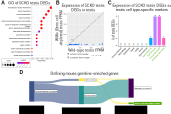
\includegraphics{../submission/compiled_figs/What_are_germline_genes.pdf}
  \caption[Aberrant transcription of germline genes in the \textit{Kdm5c}-KO in the brain]{\textbf{Aberrant transcription of germline genes in the \textit{Kdm5c}-KO in the brain.} \textbf{A.} enrichPlot gene ontology (GO) of \textit{Kdm5c}-KO amygdala and hippocampus testis-enriched DEGs \textbf{B.} Expression of testis DEGs in wild-type (WT) testis versus germ cell-depleted (W/Wv) testis. Expression is in Fragments Per Kilobase of transcript per Million mapped reads (FPKM). \textbf{C.} Number of testis DEGs that were classified as cell-type specific markers in a single cell RNA-seq dataset of the testis (Green et al 2018). Germline cell types are highlighted in green, somatic cell types in black. \textbf{D.} Sankey diagram of mouse genes filtered for germline enrichment based on their expression in wild-type and germline-depleted mice and in adult mouse non-gonadal tissues (Li et al 2017).}
  \label{figurelabel}
\end{figure}

\begin{figure}
  \centering 
  \includegraphics{../submission/compiled_figs/EpiLCs_too.pdf}
  \caption[\textit{Kdm5c}-KO epiblast-like cells express key drivers of germline identity ]{\textbf{\textit{Kdm5c}-KO epiblast-like cells express key drivers regulators of germline identity A.} Top - Diagram of \textit{in vivo} differentiation of embryonic stem cells (ESCs) of the inner cell mass into epiblast stem cells. Middle - \textit{in vitro} differentiation of ESCs into epiblast-like cells (EpiLCs). Bottom - representative images of wild-type (WT) and \textit{Kdm5c}-KO ESC to EpiLC differentiation. Brightfield images taken at 20X. \textbf{B.} No significant difference in primed pluripotency maker expression in wild-type versus \textit{Kdm5c}-KO EpiLCs. Welch's t-test, expression in transcripts per million (TPM). \textbf{C.} Number of tissue-enriched differentially expressed genes (DEGs). * p<0.05, ** p<0.01, *** p<0.001, Fisher's exact test. \textbf{D.} Average bigwigs of an example germline gene, \textit{Cyct}, that is dysregulated \textit{Kdm5c}-KO EpiLCs. \textbf{E.} Upset plot displaying the overlap of germline DEGs expressed in \textit{Kdm5c}-KO EpiLCs, amygdala (AMY), and hippocampus (HIP) RNA-seq datasets. \textbf{F.} enrichPlot comparing enriched gene ontologies for \textit{Kdm5c}-KO EpiLC, amygdala, and hippocampus germline DEGs. \textbf{G.} Top - Example germline identity DEGs unique to EpiLCs, p-values for Welch's t-test. Bottom - Average bigwigs of \textit{Dazl} and \textit{Stra8} expression in wild-type and \textit{Kdm5c}-KO EpiLCs \textbf{H.} Immunocytochemistry of DAZL in male wild-type (WT) and \textit{Kdm5c}-KO (5CKO) EpiLCs. Percentage of DAZL-positive cells normalized to DAPI, p-value for Welch's t-test.}
  \label{figurelabel}
\end{figure}

\textbackslash begin\{figure\} \centering 
\includegraphics{../submission/compiled_figs/KDM5C_ChIPseq.pdf}

\caption[KDM5C binds to a subset of germline gene promoters during early embryogenesis]{\textbf{KDM5C binds to a subset of germline gene promoters during early embryogenesis.} \textbf{A.} ChIPseeker localization of KDM5C peaks at different genomic regions in EpiLCs (top) and hippocampal and cortex primary neuron cultures (PNCs, bottom). \textbf{B.} Overlap of genes with KDM5C bound to their promoters in EpiLCs (purple) and PNCs (blue). \textbf{C.} Gene ontology comparision of genes with KDM5C bound to their promoter. Genes were classified as either bound in EpiLCs only (EpiLC only), unique to PNCs (PNC only, no significant ontologies) or bound in both PNCs and EpiLCs (shared). \textbf{D.} Average KDM5C binding at all germline-enriched genes in EpiLCs (left) and PNCs (right).\textbf{E.} KDM5C binding at the promoters of RNA-seq germline DEGs. Genes were classified as either only dysregulated in EpiLCs (EpiLC only), genes dyresgulated in the hippocampus or amygdala but not EpiLCs (brain only), or genes dysregulated in both EpiLCs and the brain (common). \textbf{F.} Example ChIP-seq bigwigs of DEGs unqiue to EpiLCs. Although both are expressed in EpiLCs, KDM5C is bound to the \textit{Dazl} promoter but not the \textit{Stra8} promoter}

in EpiLCs. \textbf{G.} Example ChIP-seq bigwigs of DEGs common between
brain and EpiLCs. KDM5C is bound to the \textit{D1Pas1} promoter but not
the \textit{XXX} promoter\} in EpiLCs. \textbf{H.} Example ChIP-seq
bigwigs of DEGs unique to the brain. KDM5C is bound to the \textit{XXX}
promoter but not the \textit{Meig1} promoter.\} \label{figurelabel}
\textbackslash end\{figure\}

\begin{figure}
  \centering
  \includegraphics{../submission/compiled_figs/KDM5C_Mechanism.pdf}
  \caption[KDM5C’s catalytic activity promotes long-term silencing of germline genes via DNA methylation]{\textbf{KDM5C’s catalytic activity promotes long-term silencing of germline genes via DNA methylation.} \textbf{A.} Left - Bigwigs of representative H3K4me3 ChIP-seq peaks in the wild-type and Kdm5c-KO adult amygdala at two germline gene promoters. \textbf{B.} Left - Bigwigs of representative H3K4me2 ChIP-seq peaks in wild-type and Kdm5c-KO EpiLC. \textbf{C.} RNA and protein expression of KDM5C across ESC to EpiLC differentiation. Top left - diagram of differentiation protocol and collection time points. Bottom left - representative lanes of KDM5C western blot with DAXX loading control. Middle - KDM5C protein expression normalized to DAXX. Quantified intensity using ImageJ (artificial units - au). Right - RT-qPCR of \textit{Kdm5c} RNA expression, calculated in comparision to TBP expression (2-deltaCT) \textbf{D.} XXX {E.} XXX.}
  \label{figurelabel}
\end{figure}

\newpage

\hypertarget{figure-outline}{%
\subsection{Figure outline:}\label{figure-outline}}

\textbf{Figure 1: Misexpression of tissue-specific genes in the
\emph{Kdm5c}-KO brain} * MA-plot and bar graphs of tissue-enriched genes
* Example testis-specific genes (NCBI and bigwigs) * An example ovary
tissue-specific gene * An example muscle/liver tissue-specific gene
(NCBI and bigwigs)

\textbf{Figure 2: The male \emph{Kdm5c}-KO brain expresses male and
female germline-enriched genes} * Gene ontology of testis DEGs in the
amygdala and hippocampus - ontologies are germline ontologies *
Expression of testis DEGs in germline-depleted testis (this is adult
testis data) * scRNAseq of testis - \# of testis DEGs that are
germline-specific markers * Although far fewer, 5CKO brain also
expresses ovary-enriched genes(NCBI and bigwigs of Zar1) * These ovary
enriched genes are also germline specific (NCBI/Li tissues are in adult
ovary, so it would be best to show they're oocyte-specific in adult
ovary. But I don't think there's a published adult female W/Wv dataset.
Could try looking at scRNAseq or just do TPM in embryonic W/Wv data
since oocytes are developed at this point? Or both?) * Defining what
is/isn't a germline gene, and which are male/female biased using
embryonic W/Wv data

\textbf{Figure 3: Kdm5c-KO epiblast-like cells express key drivers
regulators of germline identity} * A) ESC to EpiLC differentiation Left
- Morphology is unchanged, * B) 5CKO EpiLCs express EpiLC
differentiation genes similar to WT lvls * C) Male EpiLCs express
germline genes (example Cyct again) * Overlap between brain and EpiLC
germline genes - show they're mostly unique * GO of Brain and EpiLC
germline genes (meiotic enriched) * Bigwigs or TPM of master regulators
* Show that while some are also 2-cell genes (Dazl), 2-cell specific
genes aren't dysregulated (Zscan4). Important point because published
KDM5C dazl paper is saying KDM5C is a 2-cell regulator, but as far as I
can tell only genes shared between germline and 2-cell are
dysregulated.\\
* Staining of Dazl (+ Stra8 if I can get it to work)

\textbf{Figure 4: Loss of KDM5C's catalytic activity impairs DNAme
placement and long-term silencing of germline genes} * Increase in
H3K4me3 in Kdm5c-KO amygdala at germline genes * Increase in H3K4me2 in
EpiLCs at germline genes * Kdm5c binding in EpiLCs vs PNCs to show that
germline repression is happening in early embryo * Previous studies only
looked at ESCs, unknown if catalytic activity is required for long-term
repression, especially since DNA methylation is placed later). KDM5C RNA
and protein ESC --\textgreater{} EpiLC (increasing then decreasing) *
RNA expression of germline genes with catalytic dead rescue (Ilakkiya) *
DNA methylation in WT and 5CKO EpiLCs (Ilakkiya)

\textbf{Figure 5: Ectopic, germline-like phenotypes in Kdm5c-KO
ESCs/EpiLCs} * Sycp3 staining * DDX4 staining and repression of
retrotransposons * Cilia??

\end{document}
